\documentclass{beamer}
\usetheme{Singapore}
\usecolortheme{default}

\usepackage[utf8]{inputenc}
\usepackage[T1]{fontenc}
\usepackage{verbatim}
\usepackage{graphics}
\usepackage{listings}
\usepackage{lmodern}

\title{Understanding Git with Alloy}
\subtitle{Milestone 3}
\author{Cláudio Lourenço \and Renato Neves}
\institute{University of Minho\\
Formal Methods in Software Engineering}


\logo{ 
\includegraphics[width=0.15\textwidth]{images/csail_logo.png}
       
\includegraphics[width=0.15\textwidth]{images/uminho_eng_logo.png}}

\begin{document}

\frame {
   \titlepage
}

\frame{
   \frametitle{Table of contents}
   \tableofcontents 
}

\section{Git as VCS}

\begin{frame}
	\frametitle{Git as VCS}
	\begin{block}{Git is one of many Version Control Systems}
		\begin{itemize}
		\item Fast
		\item Efficient
		\item Oriented to snapshots - Not differences
		\item Widely used
	\end{itemize}
	\end{block}
\end{frame}

\section{Project Motivation and Objectives}
\begin{frame}
	\frametitle{Project Motivation}
	\begin{block}{Gap in existing Git documentation}
		\begin{itemize}
		\item Lack of precise descriptions
		\item Contradictions between manuals
		\item Git users could benefit from a manual that is precise and rigorous
	\end{itemize}
	\end{block}
\end{frame}

\begin{frame}
	\frametitle{The dark world of Git}
	\begin{block}{The common (and above average) knowledge of Git }
	\begin{itemize}
	\item "if there are any uncommitted changes when you run git checkout,
	 Git will behave very strangely." \footnote{"Understanding Git" Manual}
	\item "When you create a branch, it will contain everything
         committed on the branch you created it from at that given
         point. So if you commit more things on the master branch like
         you have done (after creating b), then switch to branch b,
         they won't appear. This is the correct behavior. Does that
         answer your question?" \footnote{An user of Git development 
	 mailing list} 
	\end{itemize}
	\end{block}
\end{frame}

\begin{frame}
	\frametitle{Objectives of this project}
	\begin{block}{Shine some light into Git internals}
		\begin{itemize}
			\item Build a precise model of how Git works using Alloy
			\item Analyze the model and verify which properties it
			does (not) guarantee
			\item Help others understanding Git, writing a new
			(hopefully more precise) manual
		\end{itemize}
	\end{block}
\end{frame}


\section{Git Internals}

\begin{frame}
   \frametitle{The Git Structure}
   \begin{figure}
      \centering
      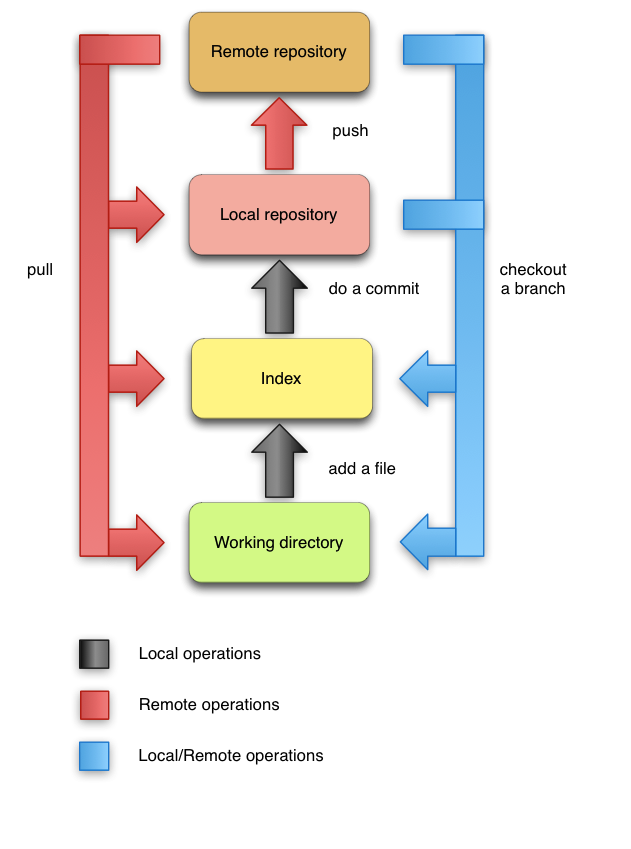
\includegraphics[width=0.45\textwidth]{images/git_workflow.png}
   \end{figure}
\end{frame}



\begin{frame}[fragile]
   \frametitle{Blob and Tree}
   \begin{block}{Blob}
      \begin{itemize}
         \item Represents the content of a file
         \item The identifier is an hash calculated from its content
         \item Files with same content will be represented by the same blob
      \end{itemize}
      \tiny
      \color{blue}
      \begin{lstlisting}
      sig Blob extends Object {}
      \end{lstlisting}
   \end{block}
   \begin{block}{Tree}
      \begin{itemize}
         \item Contains Blobs or other Trees 
         \item Used to represent the file system structure
	      \item The identifier is an hash calculated in a similar way to the Blobs
         \item Sharing is done as in Blobs - Same content, same Tree
      \end{itemize}
      \tiny
      \color{blue}
      \begin{lstlisting}
      sig Tree extends Object {
         contains: Name -> lone(Tree+Blob)
      }
      \end{lstlisting}
   \end{block}
\end{frame}

\begin{frame}[fragile]
   \frametitle{Commit}
   \begin{itemize}
      \item A snapshot of the project on a certain moment
      in time
      \item It has a set of parents, that are considered the previous commits 
	   \item Points to a Tree that represents the root folder in the
	Working Directory
      \item An auxiliary abstract relation was specified
   to simplify the commit operation
   \end{itemize}
   \tiny
   \color{blue}
   \begin{lstlisting}
                        sig Commit extends Object {
                           points : Tree,
                           parent : set Commit,
                           abs: Path -> Object,
                           merge : set State
                        }
                           
                        sig RootCommit extends Commit {}
\end{lstlisting}
\end{frame}

\begin{frame}[fragile]
\frametitle{Branch and HEAD}
   \begin{block}{Branch}
      \begin{itemize}
         \item It is just a pointer to a commit - Unlike other VCS, where a branch is a full copy of the repository
      \end{itemize}
   \end{block}
   \begin{block}{HEAD}
      \begin{itemize} 
         \item Special reference that identifies the current Branch
      \end{itemize}
   \end{block}
   \tiny
   \color{blue}
   \begin{lstlisting}
                        sig Branch{
                           marks: Commit lone -> State,
                           branches: set State,
                           head: set State
                        }

                        lone sig Master extends Branch{}
   \end{lstlisting}
\end{frame}
\begin{frame}

\frametitle{Repository}
   \begin{figure}
      \centering
      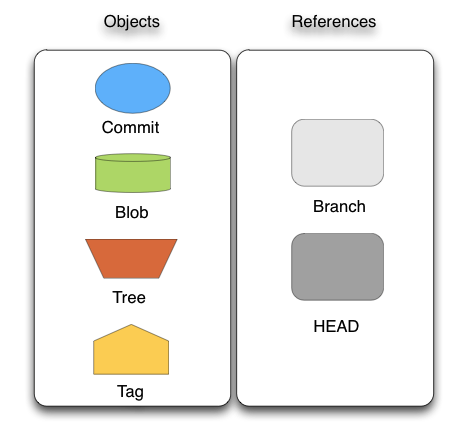
\includegraphics[width=0.5\textwidth]{images/legenda2.png}
   \end{figure}
\end{frame}

\begin{frame}
	\frametitle{Repository}
	\begin{figure}
		\centering
		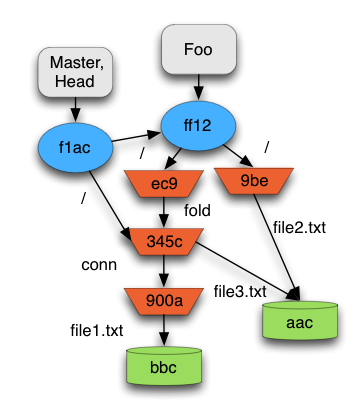
\includegraphics[width=0.4\textwidth]{images/object_assoc.png}
	\end{figure}
\end{frame}


\begin{frame}[fragile]
   \frametitle{Working Directory}
   \begin{itemize}
      \item Subset of a file system that is tracked by Git
   	\item In our model we simplify this component using the notion
      of path
	   \item Our convention dictates that if a file exists in an Alloy
	   instance, then it automatically exists in the Working Directory
   \end{itemize}
   \tiny
   \color{blue}
   \begin{lstlisting}
                        sig Path {
                           pathparent: lone Path,
                           name: Name,
                           unmerge: set State
                        }

                        one sig Root extends Path{}
   \end{lstlisting}
\end{frame}


\begin{frame}[fragile]
   \frametitle{Index}
   \begin{itemize}
      \item Contains all files that are going to be committed on the next
      commit 
      \item The index is not necessarily equal to the Working Directory
      \item If an user wants to commit a new file or a modified file,
      first he must add it to the index
   \end{itemize}
   \vspace{10mm}
   \tiny
   \color{blue}
   \begin{lstlisting}
                        sig File{
                           path: Path,
                           blob: Blob,
                           index: set State
                        }

   \end{lstlisting}

\end{frame}


\section{Specification of Operations}

\begin{frame}[fragile]
   \frametitle{Modeled Operations}
   \begin{itemize}
      \item Add and Remove
      \item Commit
      \item Branch and Branch Remove
      \item {\bf Checkout}
      \item {\bf Merge (2-way and fast-forward) }
   \end{itemize}
\end{frame}

\begin{frame}
	\frametitle{Add and remove}

	\begin{block}{Add}
	\begin{itemize}
		\item Adds a file to the index
		\item Updates the content of a file in the index
		\item Those changes will be stored in the next commit
	\end{itemize}
	\end{block}

	\begin{block}{Remove}
	\begin{itemize}
		\item Removes a file from index, and from the
		Working Directory
		\item The removed file will not be present in the next commit
	\end{itemize}
	\end{block}

\end{frame}

\begin{frame}[fragile]
   \frametitle{Add}
   \begin{figure}
      \centering
      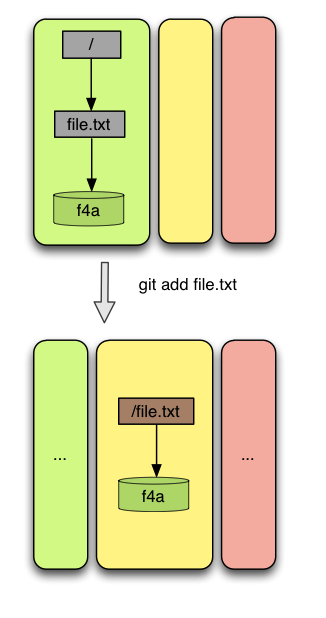
\includegraphics[width=0.3\textwidth]{images/add1.png}
   \end{figure}
\end{frame}

\begin{frame}[fragile]
   \frametitle{Remove}
   \begin{figure}
      \centering
      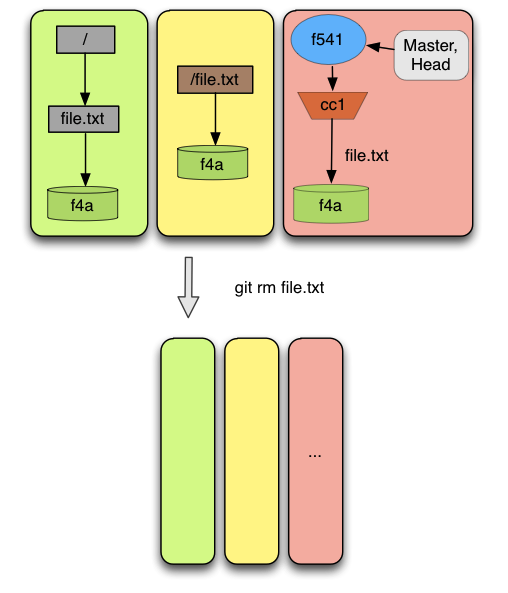
\includegraphics[width=0.45\textwidth]{images/remove1.png}
   \end{figure}
\end{frame}

\begin{frame}
	\frametitle{Commit}

	\begin{block}{Commit}
	\begin{itemize}
	\item A snapshot of a project on a certain moment in time
	\item In the first version of the model it was very difficult to
   model such operation
	\item An abstract relation was then modeled to map objects on a
   certain commit with a path
	\end{itemize}
	\end{block}

\end{frame}

\begin{frame}[fragile]
   \frametitle{Commit}
   \begin{figure}
      \centering
      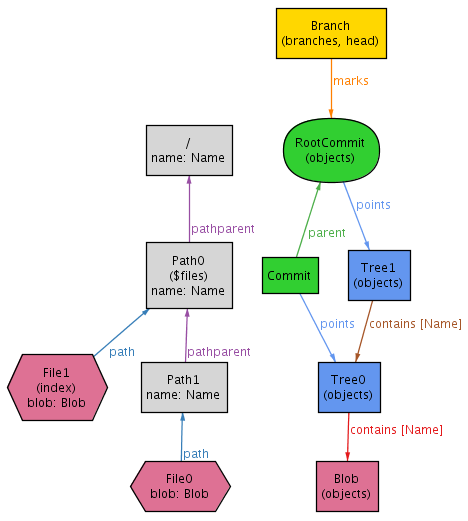
\includegraphics[width=1.0\textwidth]{images/commit1.png}
   \end{figure}
\end{frame}

\begin{frame}[fragile]
   \frametitle{Commit}
   \begin{figure}
      \centering
      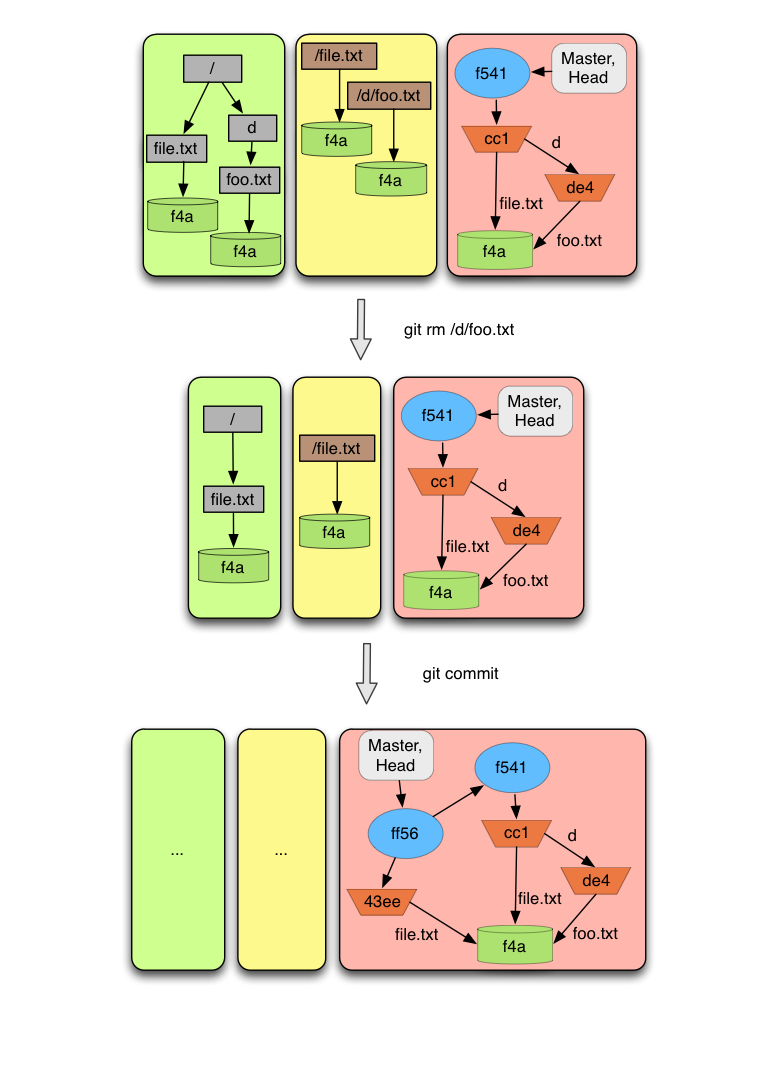
\includegraphics[width=1.0\textwidth]{images/commit2.png}
   \end{figure}
\end{frame}

\begin{frame}[fragile]
	\frametitle{Checkout}
	\begin{block}{The most difficult operation to specify}
	\begin{itemize}
		\item No manual was found with a full description
		\item No references to the existing pre-conditions - ''if there
      are any uncommitted changes when you run git checkout, Git will
      behave very strangely. The strangeness is predictable and
      sometimes useful, but it is best to avoid it...''
      \footnote{http://www.sbf5.com/~cduan/technical/git/git-2.shtml}
		\item Bug was found and reported to the Git Mailing List
      \footnote{git@vger.kernel.org}
	\end{itemize}
	\end{block}
\end{frame}

\begin{frame}
	\frametitle{Checkout pre-conditions}
	\begin{block}{Expected pre-condition}
	\begin{itemize}
		\item No uncommitted files
	\end{itemize}
	\end{block}
	\begin{block}{Real pre-condition}
	\begin{itemize}
		\item Everything that is in the index has to be
		committed, except if
		\begin{itemize}
		\item The content of a file is the same in the current
		and destination commit (warning is thrown)
		\item A file in the index does not
		exist neither in the current nor in the destination commit
		(warning is thrown)
		\item Content of a file in the index is the same as in the
		destination commit (no warning is thrown)
		\end{itemize}
	\end{itemize}
	\end{block}
\end{frame}

\begin{frame}[fragile]
   \frametitle{Checkout}
   \begin{figure}
      \centering
      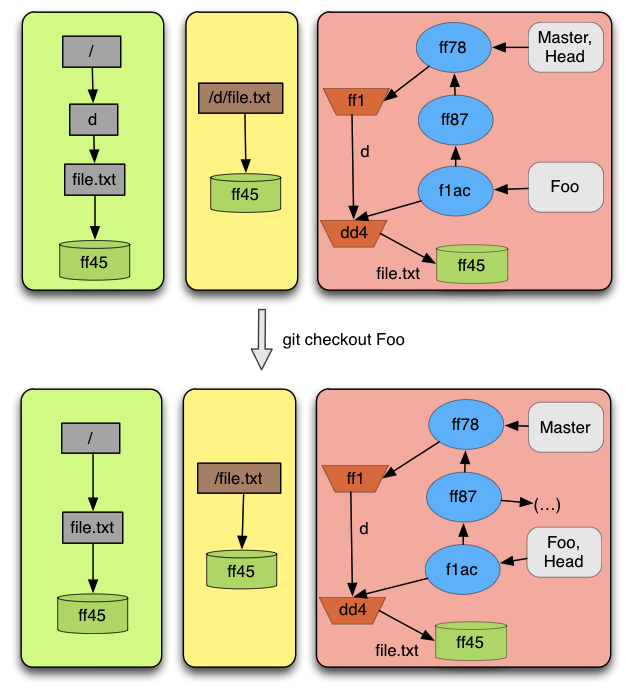
\includegraphics[width=0.50\textwidth]{images/checkout.png}
   \end{figure}
\end{frame}
\begin{frame}[fragile]
   \frametitle{Checkout}
   \begin{figure}
      \centering
      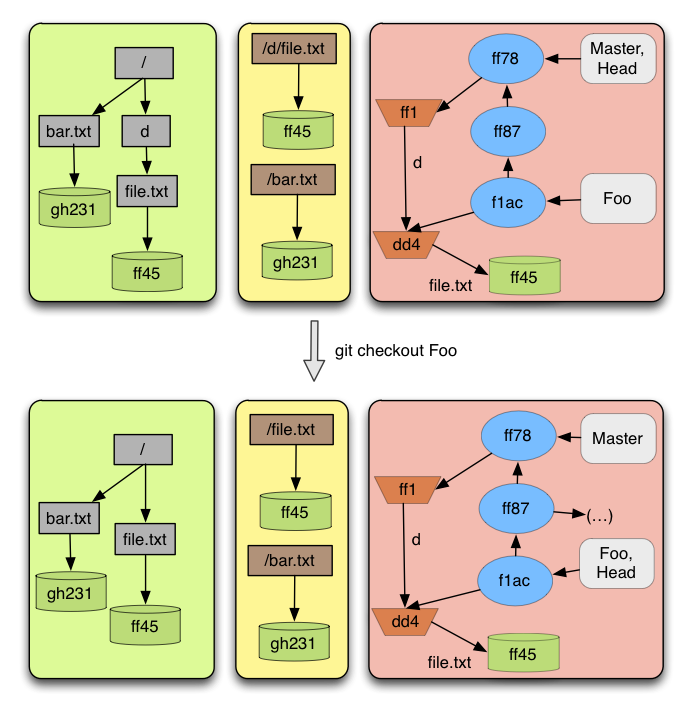
\includegraphics[width=0.55\textwidth]{images/notsosimplecheckout.png}
   \end{figure}
\end{frame}

\begin{frame}
	\frametitle{Merge }
	\begin{block}{Merge}
	   \begin{itemize}
	      \item The current commit and the commit pointed by the specified branch
	      will be merged into a possible new commit
	   \end{itemize}
	\end{block}
	\small
   \begin{block}{Merge variants}
	   \begin{itemize}
		   \item The commit being merged is more recent than
		   the current commit - A new commit is not created because the
         commit being merged takes precedence - \textbf{Fast-Forward Merge}
		   \item The typical \textbf{2-way merge} will create a new commit
		   resulting from both commits
		   \item The \textbf{3-way merge} will also create a new commit, however 
         it uses the most recent common ancestor to solve automatically 
         some conflicts that cannot be solved with 2-way merge
	\end{itemize}
	\end{block}
\end{frame}

\begin{frame}[fragile]
   \frametitle{ A fast-forward Merge}
   \begin{figure}
      \centering
      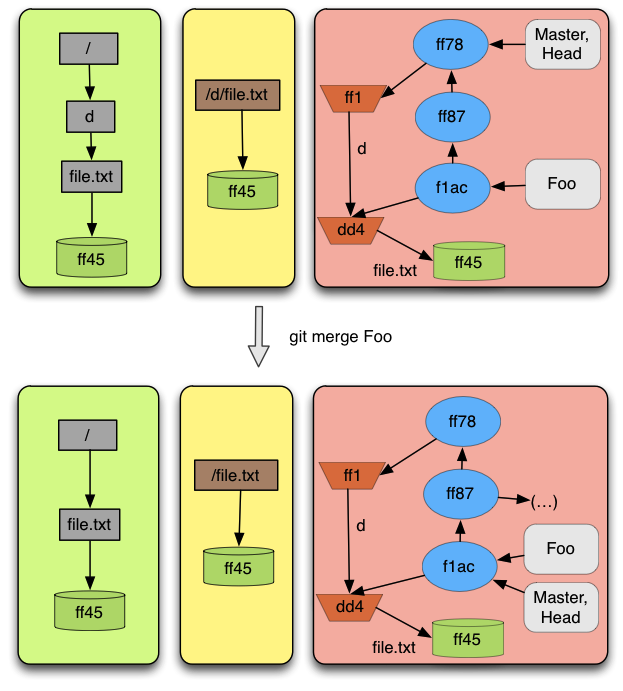
\includegraphics[width=0.50\textwidth]{images/fastforwardmerge.png}
   \end{figure}
\end{frame}

\begin{frame}[fragile]
   \frametitle{A 2-way Merge}
   \begin{figure}
      \centering
      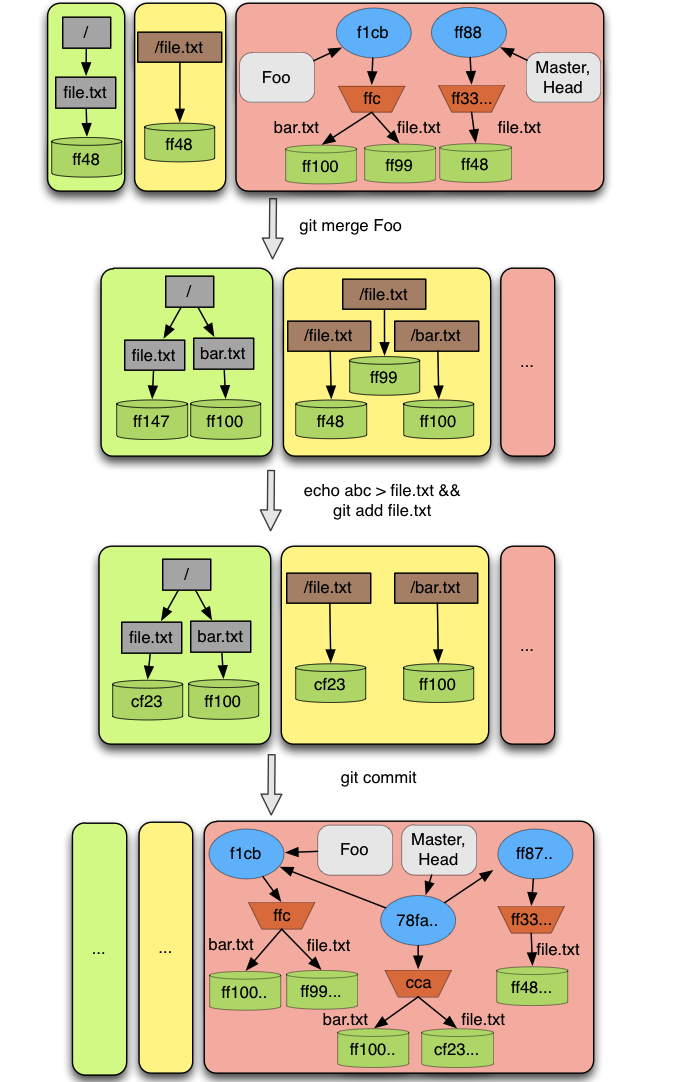
\includegraphics[width=1.0\textwidth]{images/merge2way.png}
   \end{figure}
\end{frame}

\begin{frame}[fragile]
   \frametitle{A 3-way Merge}
   \begin{figure}
      \centering
      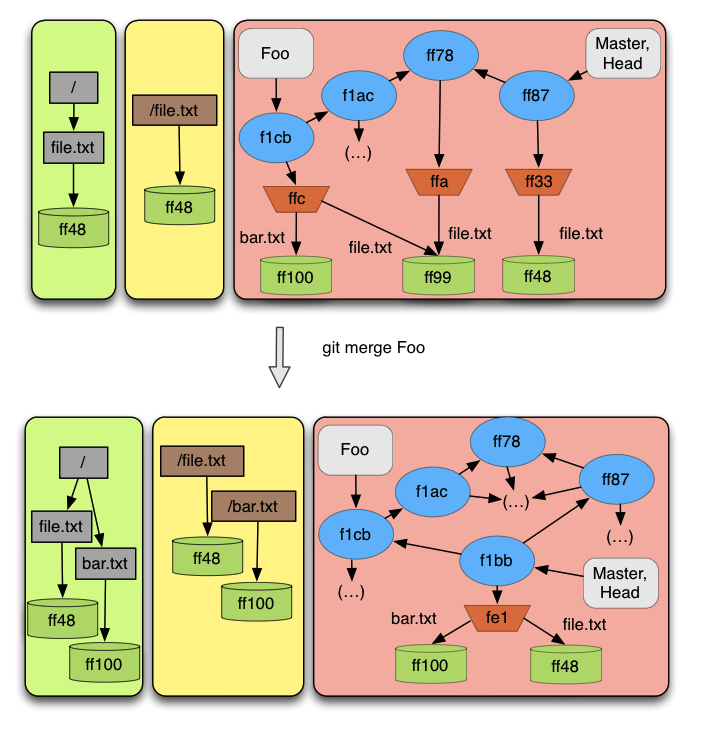
\includegraphics[width=0.55\textwidth]{images/merge3way.png}
   \end{figure}
\end{frame}

\begin{frame}[fragile]
	\frametitle{Merge specification}
   \normalsize
	\begin{itemize}
      \item Fast-Forward Merge and 2-way Merge are modeled
	   \item 3-way Merge partially modeled
	   \item Two relations had to be created for the case a manual
      merge takes place:
	   \begin{itemize}
		   \item Unmerged Files
		   \item A relation to identify the branch being merged
	   \end{itemize}
	\end{itemize}
\end{frame}

\begin{frame}[fragile]
	\frametitle{Merge specification}
	\begin{block}{Most important pre-conditions specified}
	\begin{itemize}
		\item The current commit cannot be more recent than the commit
		being merged
		\item There cannot be an unfinished merge
		\item When the fast-forward variant is applied, the index cannot have
		uncommitted files that would conflict with files from the 
		resulting merge
		\item When a 2-way or 3-way merge is applied, it is not possible
		to have uncommitted files in the index
	\end{itemize}
	\end{block}


\end{frame}

\begin{frame}
	\frametitle{Some properties checked}

	\begin{itemize}
		\item Invariant preservation 
		\item Idempotence
		\item Trees without sons
		\item No lost files on a checkout
		\item Check that one sequence of operations is in fact the
		inverse of another
	\end{itemize}
\end{frame}
\section{Documentation}

\begin{frame}
	\frametitle{Website}
	\begin{itemize}
	\item A manual was created using the knowledge obtained
	\item Website was created based on the manual 
	\item Project documentation is also available
	\item \url{http://nevrenato.github.com/CSAIL\_Git}
	\end{itemize}

\end{frame}

\section{Conclusion}

\begin{frame}
	\frametitle{Future Work}
	\begin{itemize}
	\item Model some more operations: 3-way merge, rebase, fetch, etc. 
	\item Check for some more properties that the model does (not) guarantee
	\item Build interactive diagrams of concrete examples of operations 
	\end{itemize}
\end{frame}

\begin{frame}
	\frametitle{Conclusions}
	\begin{itemize}
	\item Not enough time (not even close) to specify the whole Git
	\item It would be nice to check the properties in a theorem prover, in
	order to have completeness
	\item Model is stable and documented enough to be extended with other operations by outsiders
	\end{itemize}
\end{frame}


\end{document}
